%! Author = adrienkoumgangtegantchouang
%! Date = 08/06/25


\chapter{Requirements Analysis}\label{ch:requiremnts-analysis}


\section{Problem Statement}\label{sec:problem-statement}

With the exponential growth of online content, users are overwhelmed by the volume of news available across platforms.
This leads to difficulty in identifying relevant and trustworthy information.
The proposed system aims to aggregate articles from various news APIs and personalize the reading experience based on user behavior and preferences, while maintaining scalability and high performance.


\section{Stackeholders and Actors}\label{sec:stackeholders-actors}

The successful deployment and functioning of the Smart News Aggregator \& Reader Personalization Platform depends on multiple stakeholders and actors who interact directly or indirectly with the system.
This section outlines their roles and responsibilities.

\subsection{Stackeholders}\label{subsec:stackeholders}

\begin{itemize}
    \item \textbf{End Users}: Consume and interact with news content; expect personalized and relevant information.
    \item \textbf{Platform Administrator}: Oversees user activity, ensures data integrity, and manages access or moderation tasks.
    \item \textbf{Project Developers}: Build and maintain the system backend, frontend, and data processing pipelines.
    \item \textbf{External API Providers}: Supply news content (e.g., NYTimes, Guardian, NewsData, CurrentsAPI, MediaStack).
    \item \textbf{Academic Supervisors}: Oversee the project's architecture, correctness, and evaluate its educational objectives.
\end{itemize}

\subsection{Actors}\label{subsec:actors}

\begin{itemize}
    \item \textbf{Visitor (Anonymous user)}: Accesses the welcome page and Can register to become a user.
    \item \textbf{Registered User}: Logs into the platform, Personalizes preferences, Views news feed and Interacts with articles (like/comment).
    \item \textbf{Administrator}: Manages users and platform configurations and Monitors logs and analytics.
    \item \textbf{News Aggregator Service}: Fetches articles from external APIs and Normalizes and stores them into MongoDB.
    \item \textbf{External News APIs}: Provide raw article data in JSON format for ingestion by the system.
\end{itemize}

Each actor has specific actions and permissions that are further detailed in the Use Case and UML Diagrams.


\section{Functional Requirements}\label{sec:functional-requirments}

The Smart News Aggregator \& Reader Personalization Platform offers a suite of functionalities that serve both user-facing and administrative purposes.
The following functional requirements have been identified:

\subsection{User Account Management}\label{subsec:user-account-management}

\begin{itemize}
    \item \textbf{Registration}: Users must be able to register with valid email and password.
    \item \textbf{Login/Logout}: Authenticated access via JWT-based login; logout clears session on frontend.
    \item \textbf{Profile Management}: Users can update personal data (e.g., name, preferences).
    \item \textbf{Password Handling}: Secure password storage and update with history tracking.
\end{itemize}

\subsection{News Aggregation \& Display}\label{subsec:news-aggregation-diplay}

\begin{itemize}
    \item \textbf{Fetch Articles from External APIs}: The system retrieves and normalizes article data from third-party providers such as NYTimes, NewsData, CurrentsAPI, etc.
    \item \textbf{Categorized News Display}: Articles are displayed by category (e.g., politics, tech, sports).
    \item \textbf{Search \& Filter}: Users can search articles using keywords and filter by category, source, or date.
    \item \textbf{Pagination}: Article lists are paginated to handle large datasets.
\end{itemize}

\subsection{Personalization \& Recommendation}\label{subsec:personalization-recommendation}

\begin{itemize}
    \item \textbf{Save Preferences}: Users can set preferred categories, sources, or languages.
    \item \textbf{Personalized Feed}: Articles are filtered and ranked based on user preferences.
    \item \textbf{Like \& Save Articles}: Users can like or save articles for future reading.
    \item \textbf{Commenting System}: Users can add comments and replies to articles.
\end{itemize}

\subsection{Admin \& Analytics}\label{subsec:admin-analytics}

\begin{itemize}
    \item \textbf{Dashboard Access}: Admin can view usage statistics and system logs.
    \item \textbf{User Management}: Admin can deactivate or delete user accounts.
    \item \textbf{API Health Monitoring}: Admin is notified of errors when external APIs fail.
    \item \textbf{Article Quality Control}: Admin can remove duplicated or malformed articles.
\end{itemize}

\subsection{System \& Logging}\label{subsec:system-logging}

\begin{itemize}
    % \item \textbf{API Logging}: All requests to critical endpoints are logged (including metadata like headers and response time).
    \item \textbf{Authentication Event Logs}: Login/Logout attempts are store for audit.
    \item \textbf{Error Tracking}: Failed requests or errors are stored in MongoDB.
\end{itemize}


\section{Non-Functional Requirements}\label{sec:non-functional-requirements}

This section outlines the quality attributes and constraints the Smart News Aggregator \& Reader Personalization Platform must meet to ensure reliability, security, and scalability.

\subsection{Performance}\label{subsec:performance}

The system must handle a high number of concurrent users with minimal latency.
Article feed pages must load within 1 second under normal network conditions.
External API data must be cached using Redis to reduce response time and load.


\subsection{Scalability}\label{subsec:scalability}

The backend architecture must support horizontal scaling to accommodate growing numbers of users and API integrations.
MongoDB and Redis must be configured to handle large-scale document and key-value datasets efficiently.

\subsection{Availability}\label{subsec:availability}

The application must ensure high availability (99.9\%) during user access hours.
In the case of third-party API failure, the system should provide fallback responses or cached data when available.

\subsection{Security}\label{subsec:security}

User authentication must use JWT with asymmetric encryption (RS256).
Passwords must be securely hashed (using bcrypt) and stored with history to prevent reuse.
All endpoints must enforce token validation for sensitive operations.
Cross-Origin Resource Sharing (CORS) must be properly configured to restrict access to allowed domains.

\subsection{Maintainability}\label{subsec:maintainability}

The system must be modular, separating concerns by feature (auth, articles, users).
Logging and exception handling must be centralized to simplify debugging and maintenance.
Code must be written following best practices and TypeScript (frontend) and Python (backend) style guides.

\subsection{Usability}\label{subsec:usability}

The frontend must offer an intuitive user interface with minimal learning curve.
Responsive design must ensure accessibility on desktops, tablets, and mobile devices.

\subsection{Portability}\label{subsec:portability}

The application must run on Unix-based systems and be container-ready (Docker-compatible).
APIs must be documented using Swagger/OpenAPI to allow easy integration by external systems.


\section{Use Case Diagrams}\label{sec:use-case-diagrams}

These diagrams were created using PlantUML\@.

%\begin{figure}[!h]
%    \centering
%    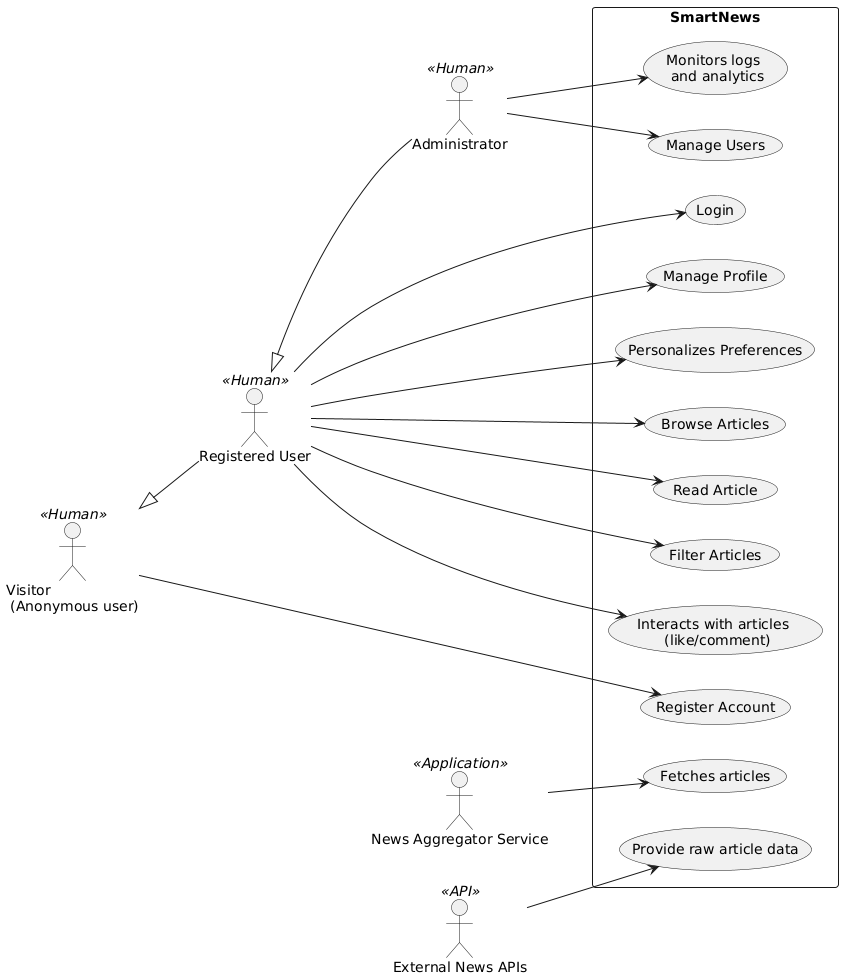
\includegraphics[width=1.1\textwidth]{chapters/chapter_02/diagram-sn-uml-2}
%    \caption{Use Case Diagram}
%    \label{fig:use-case-diagram}
%\end{figure}


\begin{figure}[!h]
    \centering
    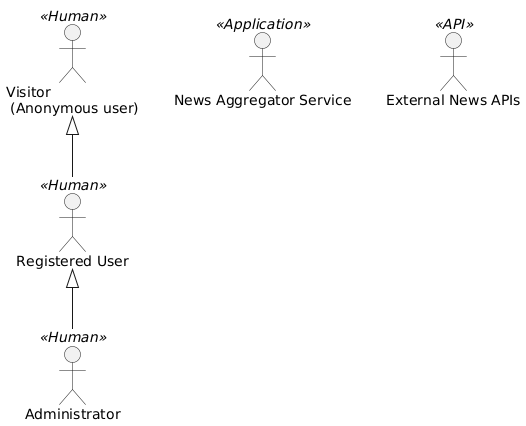
\includegraphics[width=0.5\textwidth]{chapters/chapter_02/use-case-smart-news-actors}
    \caption{Use Case Diagram : Actors}
    \label{fig:use-case-diagram-actors}
\end{figure}


\begin{figure}[!h]
    \centering
    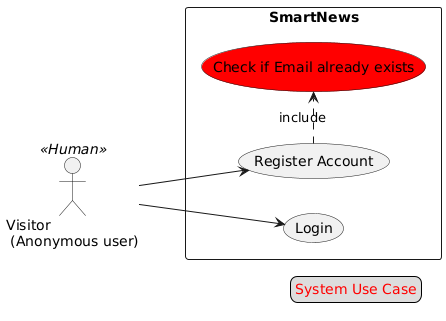
\includegraphics[width=0.5\textwidth]{chapters/chapter_02/use-case-smart-news-anonymous-user}
    \caption{Use Case Diagram: Anonymous User}
    \label{fig:use-case-diagram-anonymous-user}
\end{figure}


\begin{figure}[!h]
    \centering
    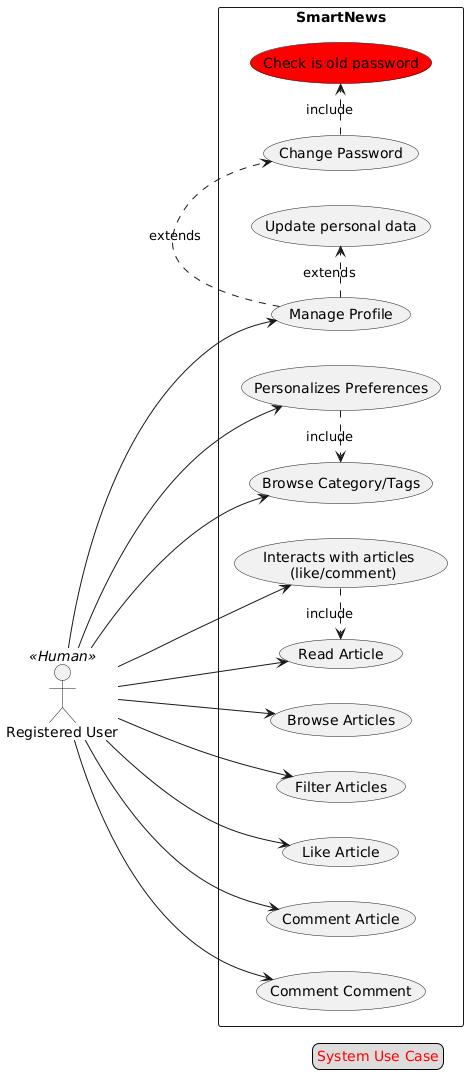
\includegraphics[width=0.5\textwidth]{chapters/chapter_02/use-case-smart-news-registered-user}
    \caption{Use Case Diagram: Registered User}
    \label{fig:use-case-diagram-registered-user}
\end{figure}


\begin{figure}[!h]
    \centering
    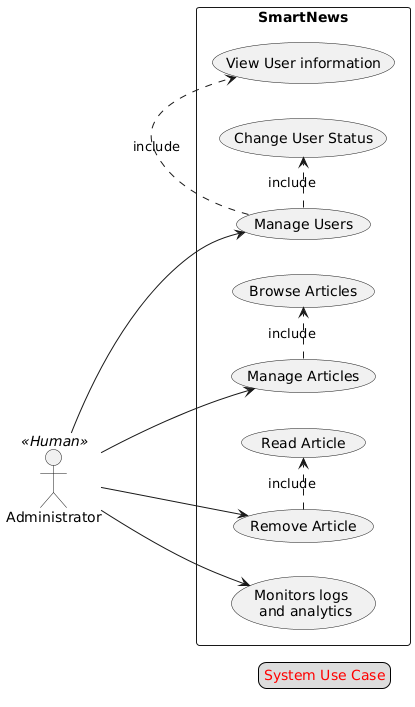
\includegraphics[width=0.5\textwidth]{chapters/chapter_02/use-case-smart-news-administrator}
    \caption{Use Case Diagram: Administrator}
    \label{fig:use-case-diagram-administrator}
\end{figure}


\begin{figure}[!h]
    \centering
    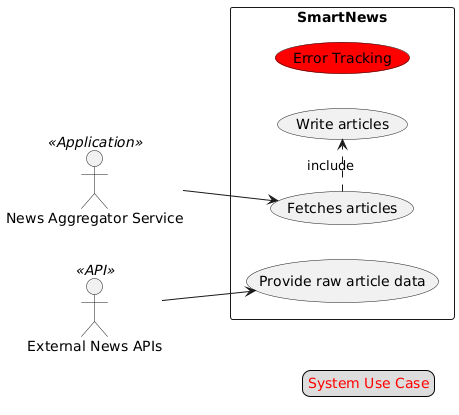
\includegraphics[width=0.5\textwidth]{chapters/chapter_02/use-case-smart-news-system}
    \caption{Use Case Diagram: Systen}
    \label{fig:use-case-diagram-system}
\end{figure}



